Each of the measured \Acpprime values from the combined lepton+jets channel is divided by the dilution factor for that CP observable to obtain the corrected asymmetry \Acp.
These values are independent of any detector or reconstruction bias and can therefore be used to search for CPV in the top quark sector.
The constraints on the dimensionless CEDM \dtG are determined based on the \Acp value of each CP observable, and are then combined using the best linear unbiased estimator method~\cite{LYONS1988110}, taking into account the correlation of the \dtG measurements among the CP observables.
The correlations between each observable pair are studied with a pseudo experiement, where 4000 sets of pseudo datasets are generated under the distribution of each observable pair.
The results are displayed in Fig.~\ref{fig:dtG_correlations}.
Most of the \dtG correlation coefficient values between the CP observables are negligible, except for the one between \Othree and \Osix, which is around 0.44.
The variation of the correlation from each systematic sources are smaller than $10^{-4}$ in the final combined \dtG.
Since there is no statistically significant evidence of CPV for any CP observable, the expected dilution factor \dilution from the SM simulation given in Table~\ref{tab:dilution_factor} is used to convert the measured \Acpprime for each CP observable to the corresponding \Acp value.
Since the unbiased estimator method only uses symmetric uncertainties, the larger of the plus and minus uncertainties in \Acpprime is taken in each case.


\begin{figure}[!th]
    \centering
    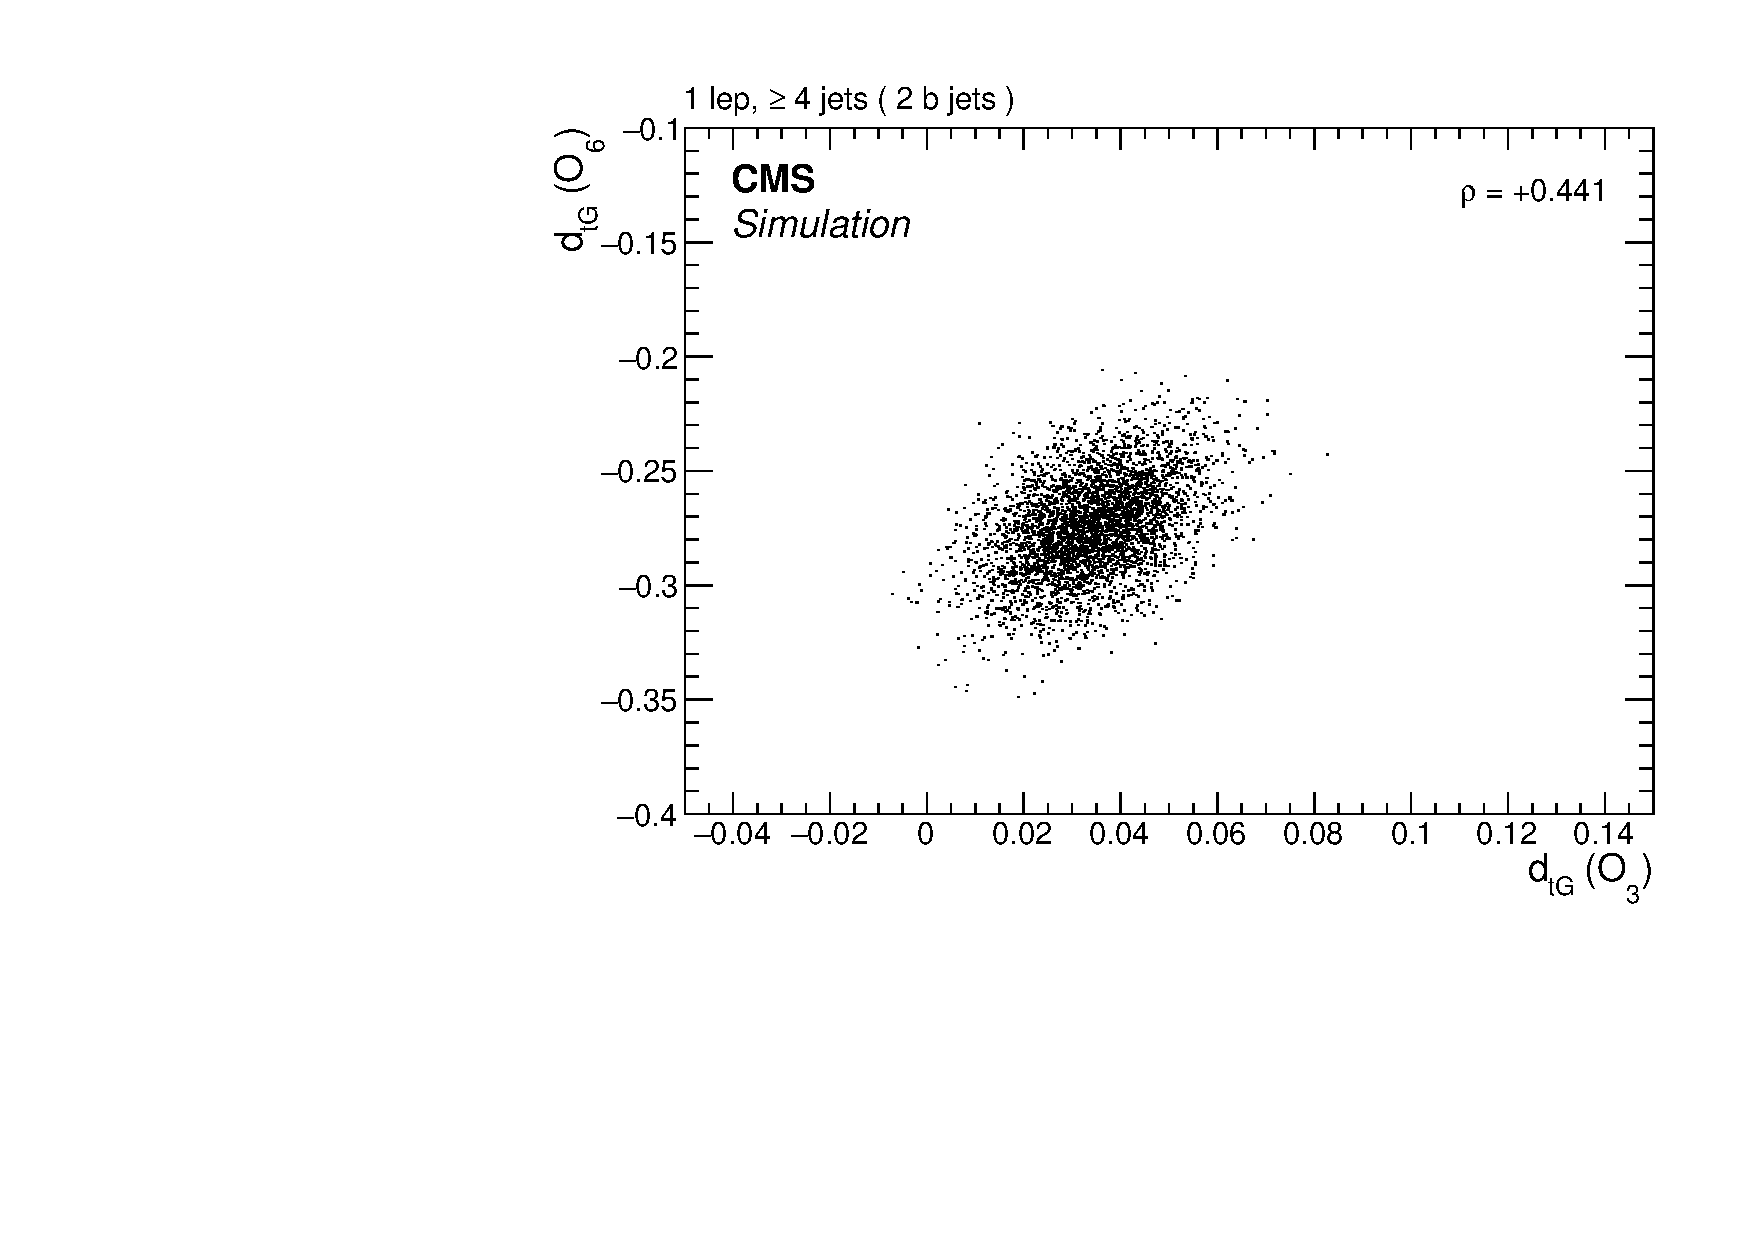
\includegraphics[width=0.45\textwidth]{figure/Corr_Sim_co_obs3_6.pdf}
    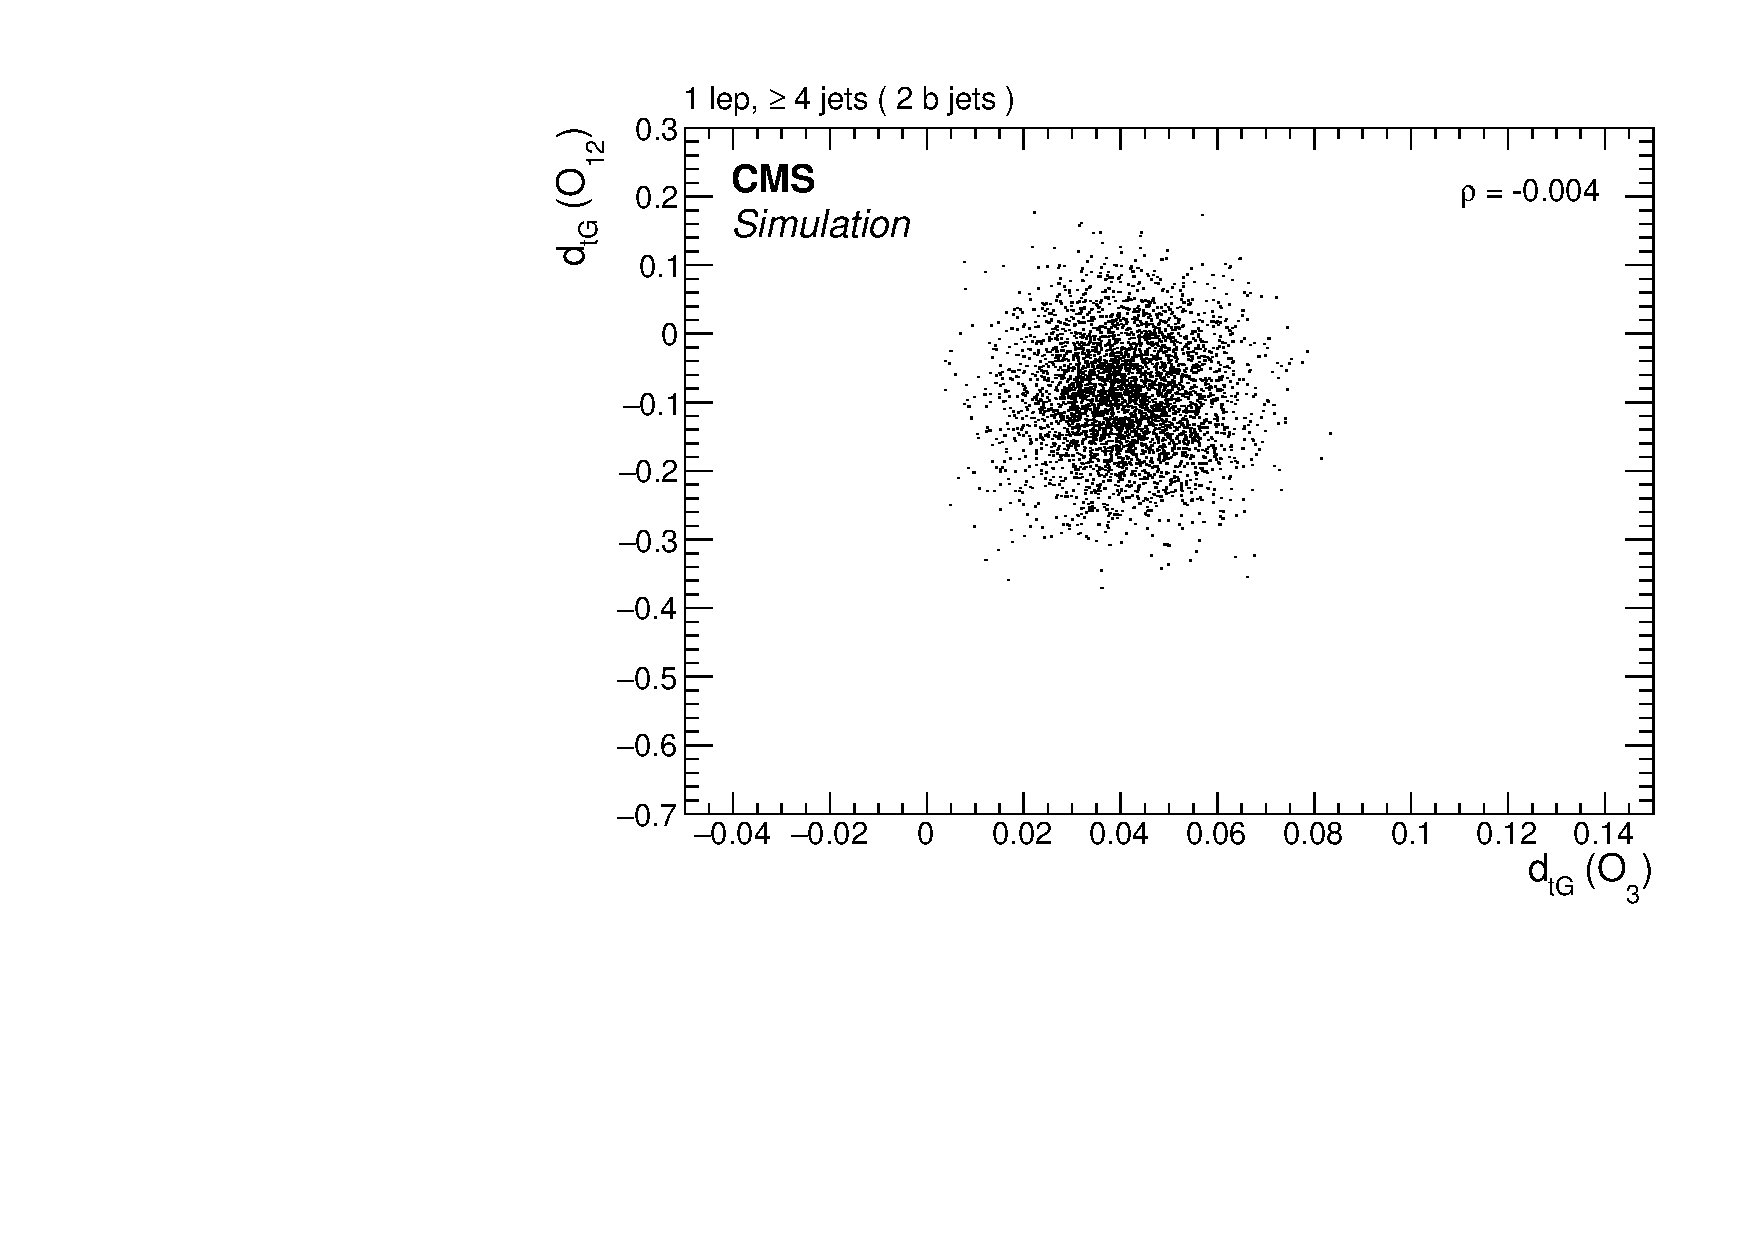
\includegraphics[width=0.45\textwidth]{figure/Corr_Sim_co_obs3_12.pdf}
    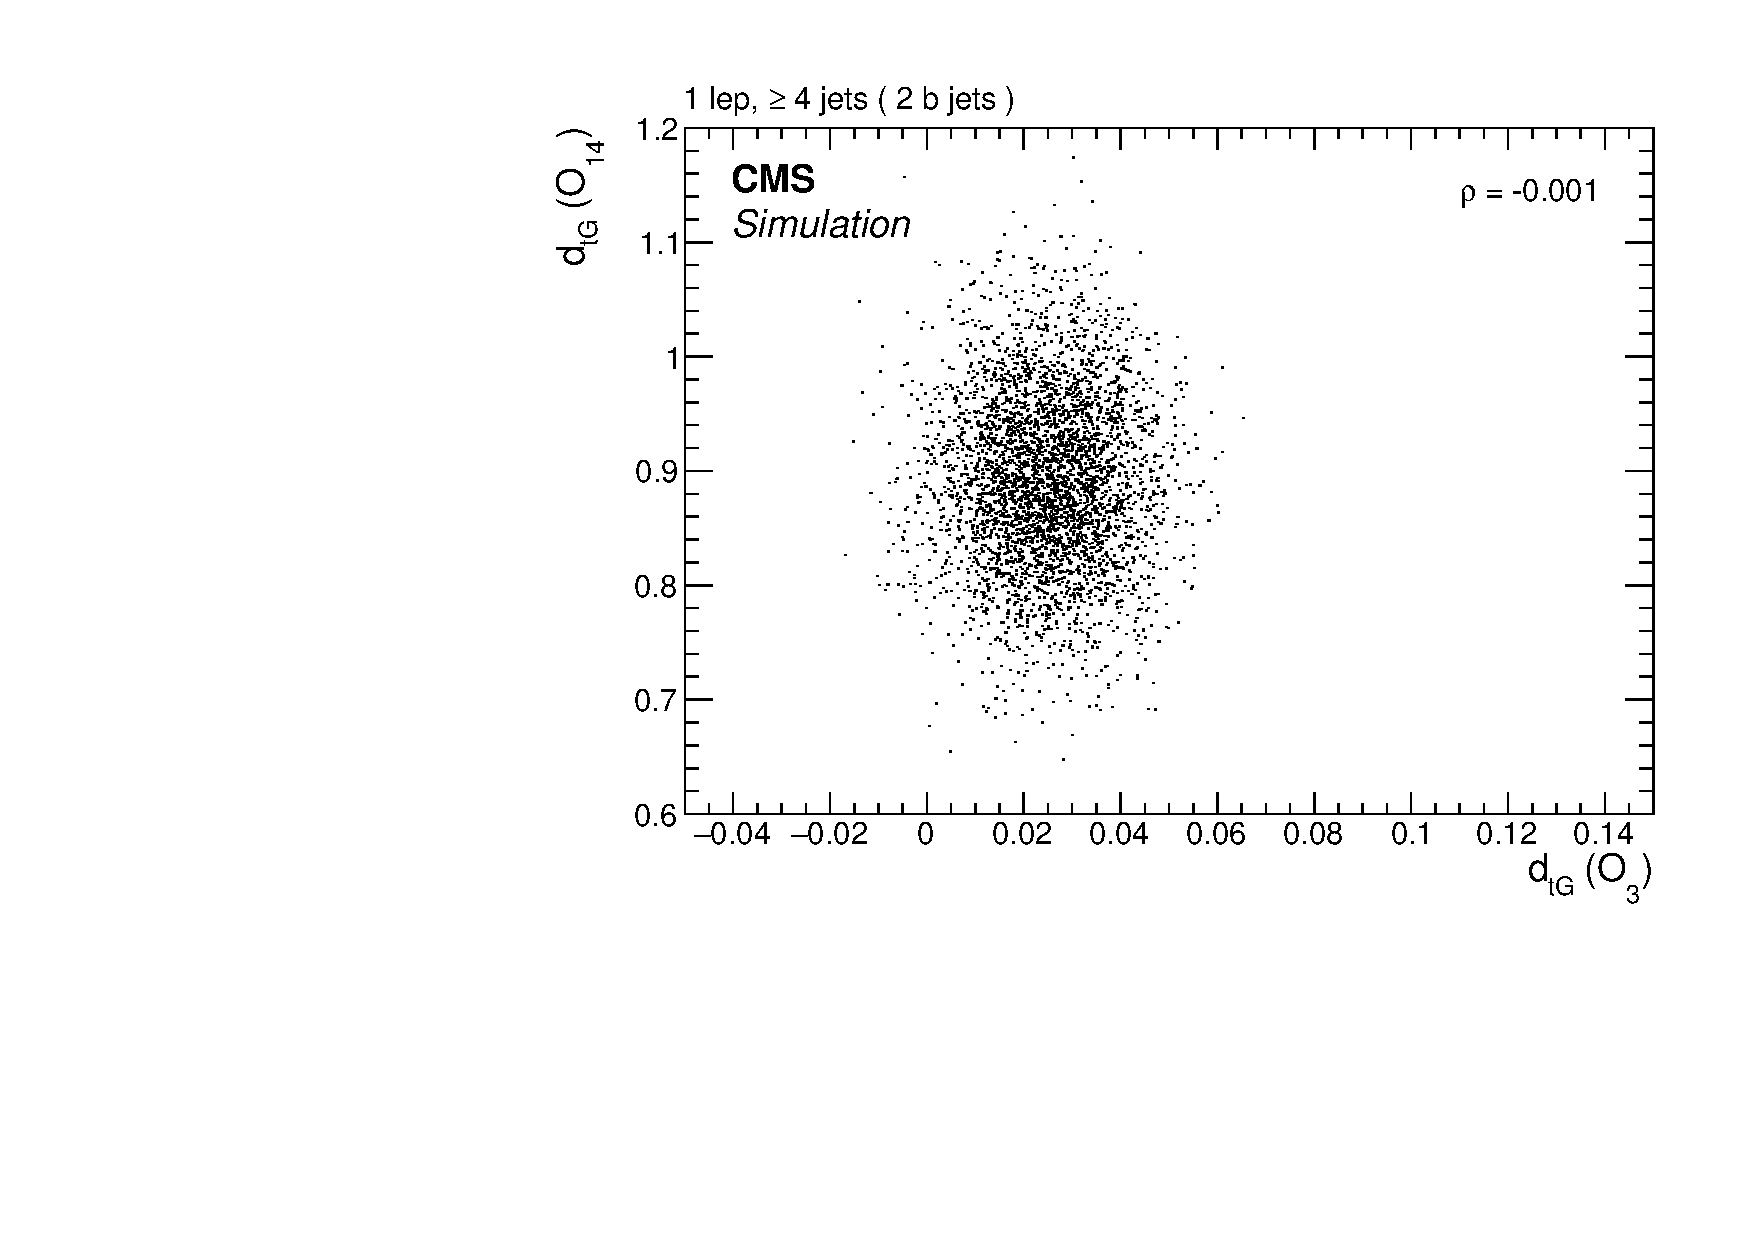
\includegraphics[width=0.45\textwidth]{figure/Corr_Sim_co_obs3_14.pdf}
    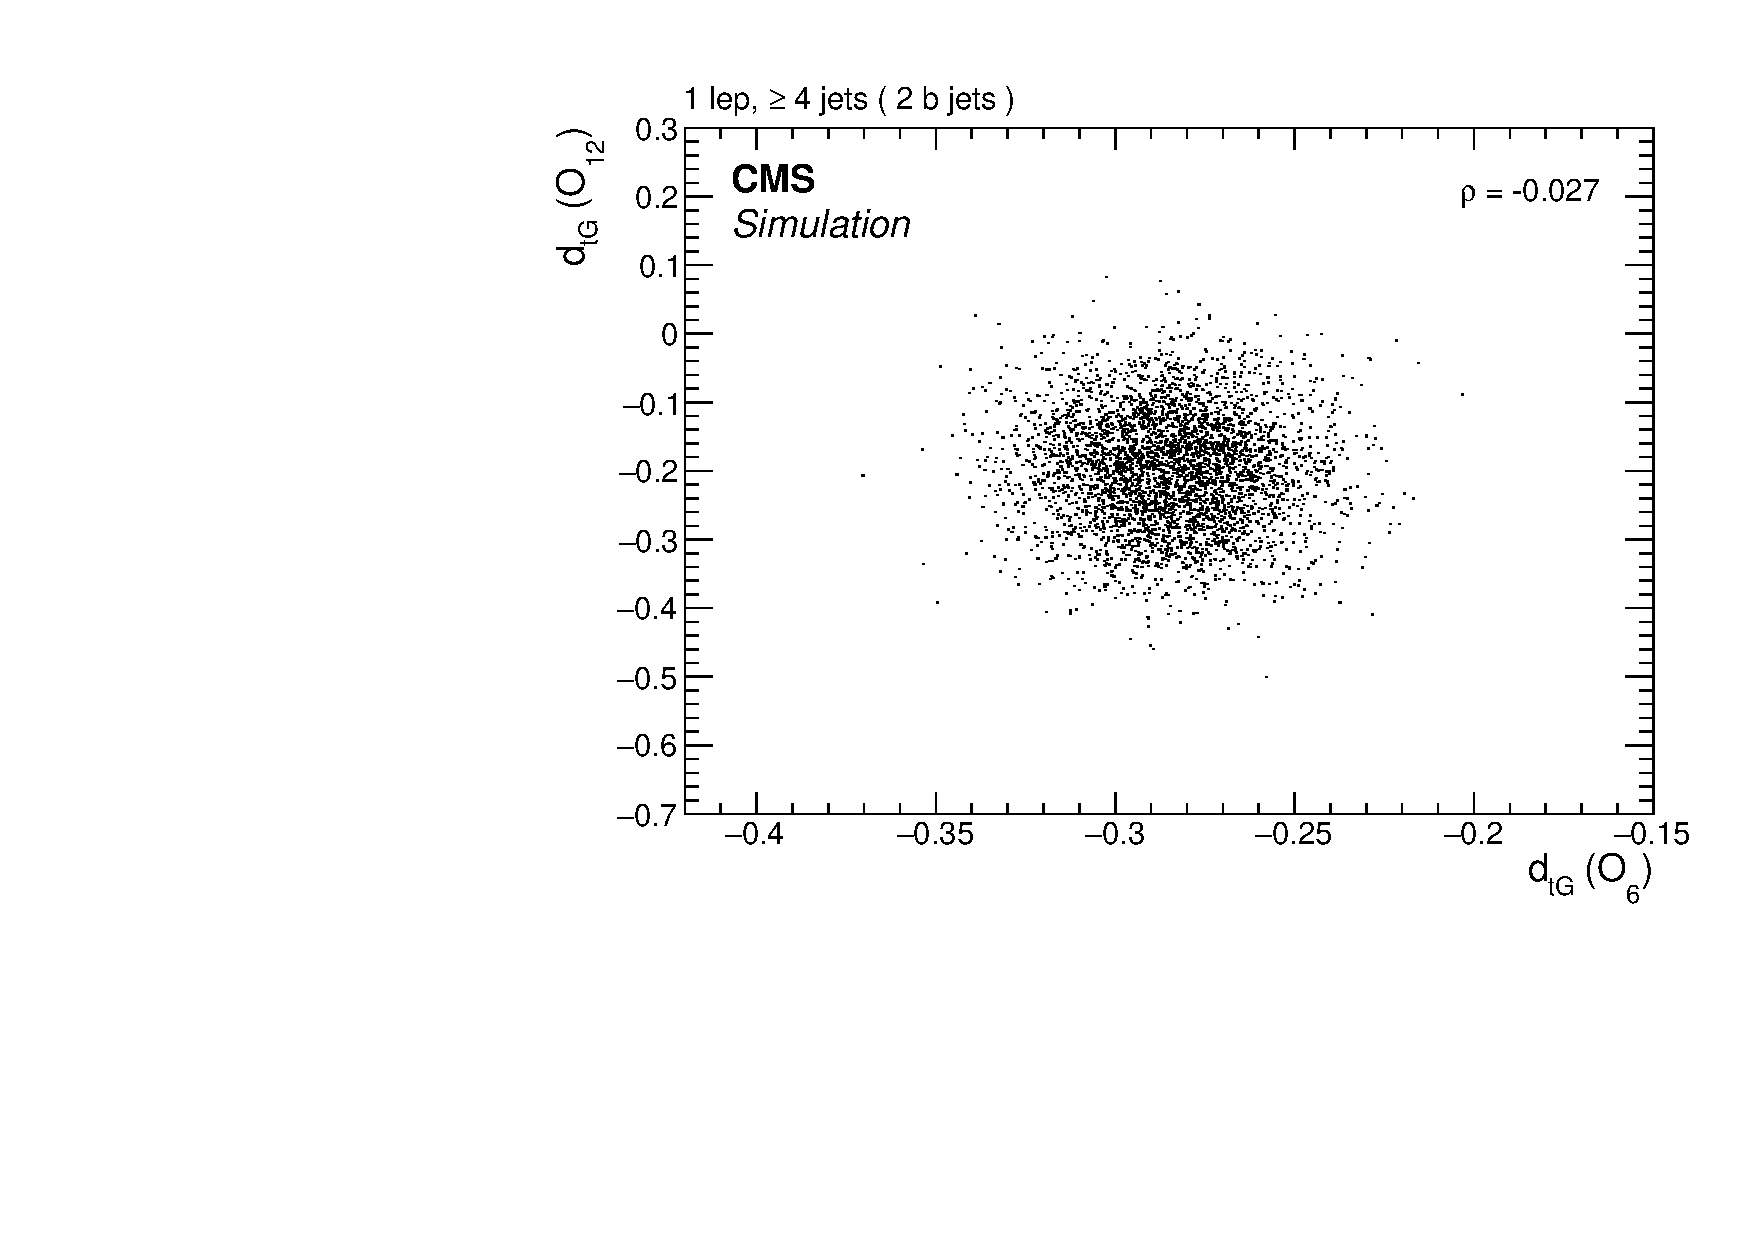
\includegraphics[width=0.45\textwidth]{figure/Corr_Sim_co_obs6_12.pdf}
    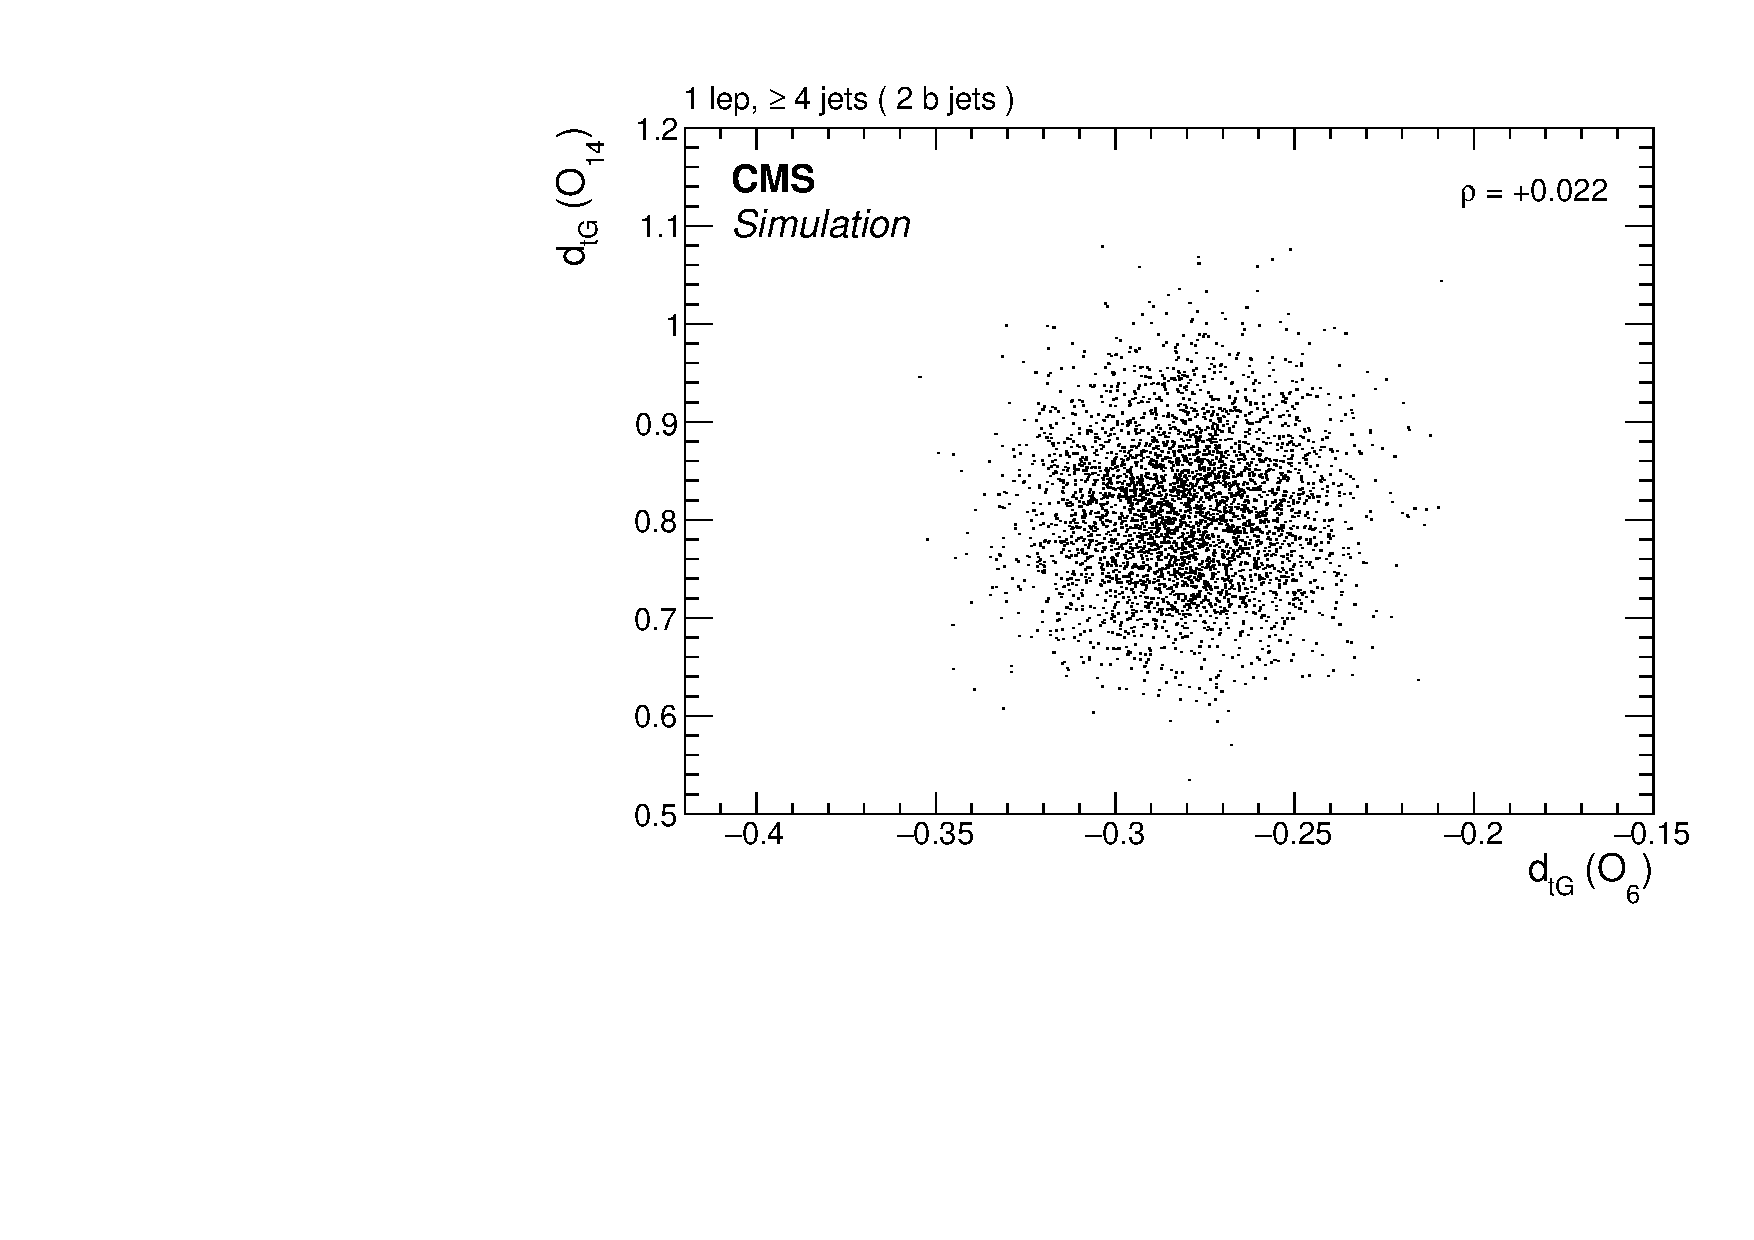
\includegraphics[width=0.45\textwidth]{figure/Corr_Sim_co_obs6_14.pdf}
    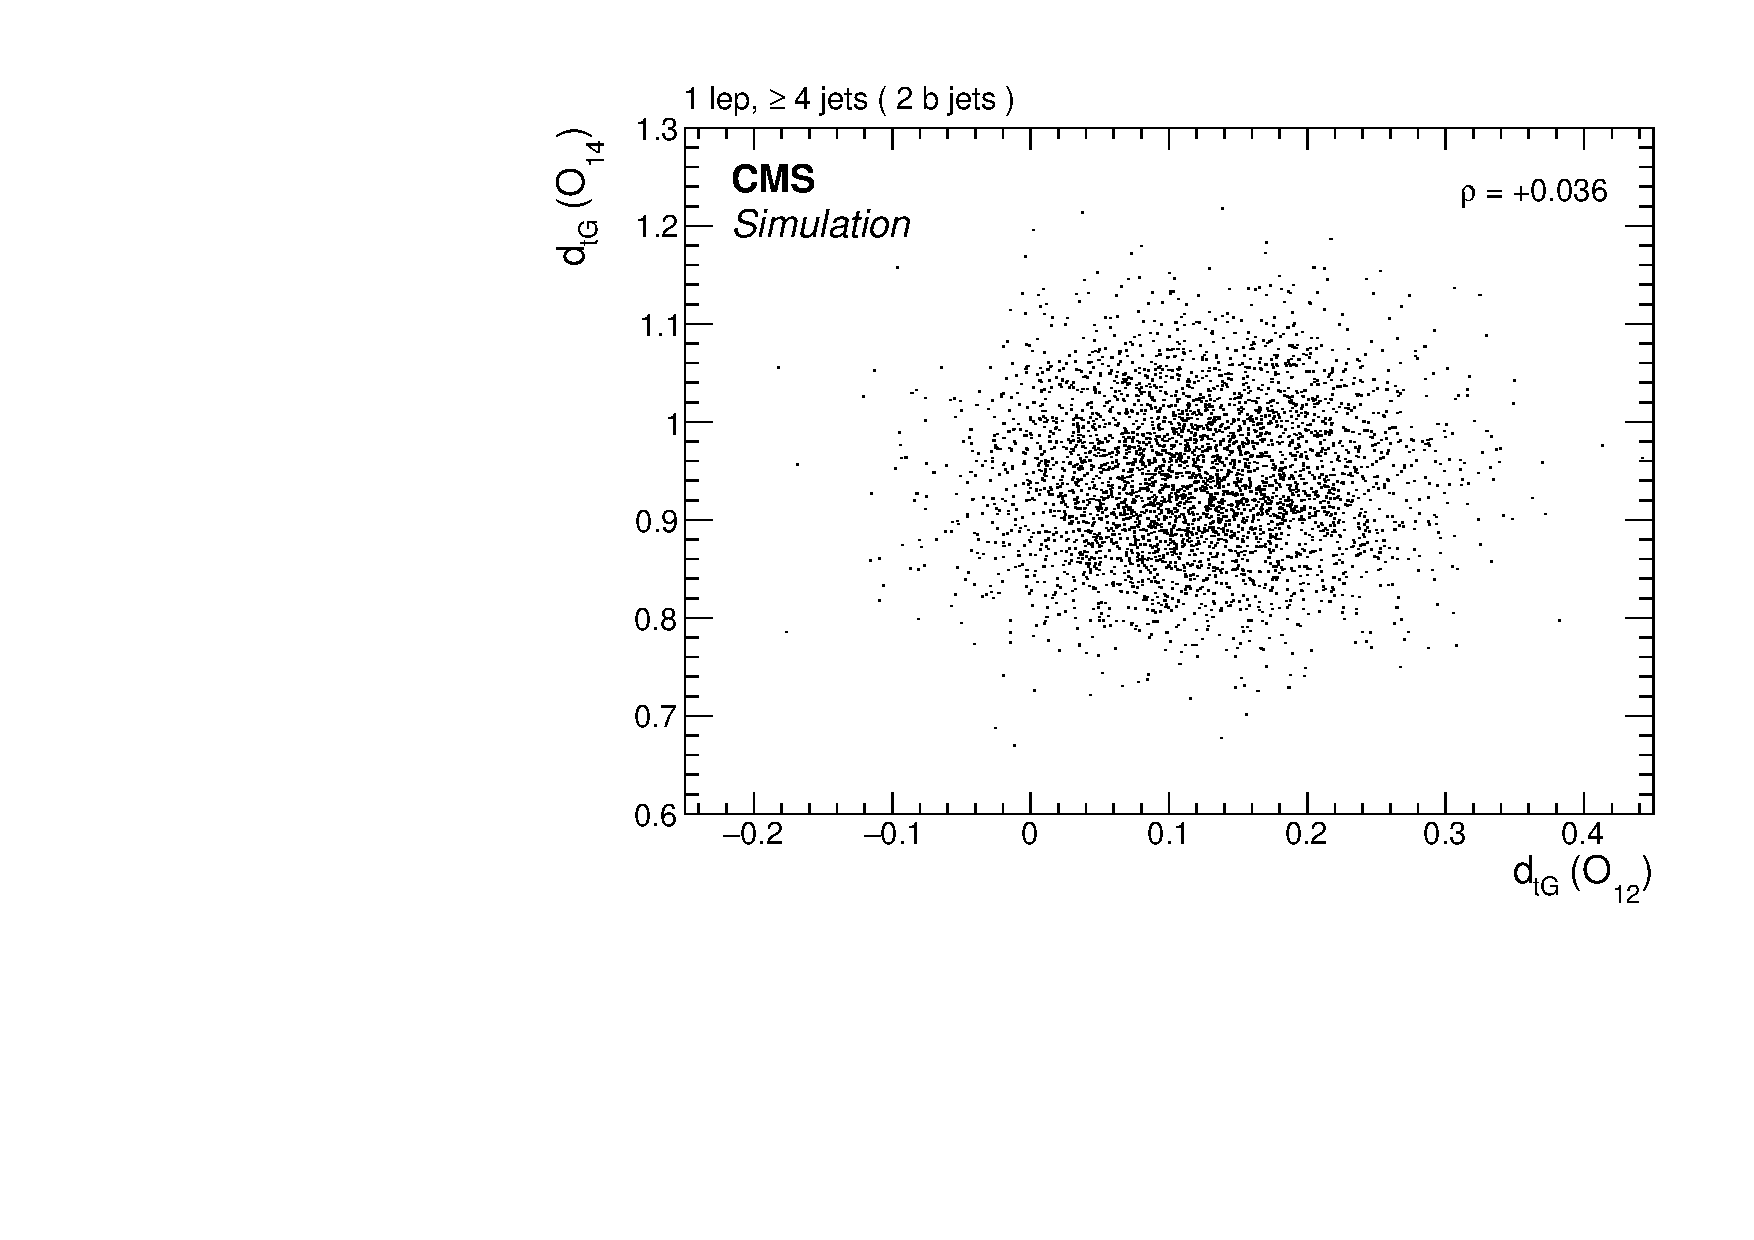
\includegraphics[width=0.45\textwidth]{figure/Corr_Sim_co_obs12_14.pdf}
    \caption[The results of the correlation of the \dtG across each observable pair.]
    {
        The results of the correlation of the \dtG across each observable pair for the combined lepton+jets channel.
        The correlation values are listed in the top-right of each plots.
    }
    \label{fig:dtG_correlations}
\end{figure}

Dedicated CP-violating \ttbar samples using the modified top quark production vertex described by Eq.~\eqref{eq:lagrangian} are simulated with different \dtG values at the generator level with \MADGRAPH to determine the relationship between \Acp and \dtG.
This relationship is parametrized by the function~\cite{CPVtop:13TeVRef}
\begin{linenomath}\begin{equation}
    \Acp = \frac{\dtG+a}{b \dtG^2+ c \dtG + d},
\end{equation}\end{linenomath}
where the parameters $a$, $b$, $c$, and $d$ are taken from a \chisq fit to the \Acp and \dtG values obtained from the different CP-violating samples.

From this relation, the dimensionless CEDM parameter \dtG is obtained from the measured \Acp value, and the uncertainty in \dtG is calculated using the full covariance matrix from the fit:
\begin{linenomath}\begin{equation}
\DsqdtG=\delvec^{T} \begin{pmatrix}
    \DsqAcp & 0 & 0 & 0 & 0 \\
    0 & \Dsqa & \mathrm{cov}(a,b) & \mathrm{cov}(a,c) & \mathrm{cov}(a,d) \\
    0 & \mathrm{cov}(b,a) & \Dsqb & \mathrm{cov}(b,c) & \mathrm{cov}(b,d) \\
    0 & \mathrm{cov}(c,a) & \mathrm{cov}(c,b) & \Dsqc & \mathrm{cov}(c,d)\\
    0 & \mathrm{cov}(d,a) & \mathrm{cov}(d,b) & \mathrm{cov}(d,c) & \Dsqd\\
\end{pmatrix} \delvec,
\end{equation}\end{linenomath}
where \DsqdtG, \DsqAcp, \Dsqa, \Dsqb, \Dsqc, and \Dsqd are the variances in \dtG, \Acp, $a$, $b$, $c$, and $d$, respectively.

The resulting CP-violating asymmetry \Acp and the dimensionless CEDM \dtG, with their statistical and systematic uncertainties, are shown in Table~\ref{tab:upper_limit} for each of the CP observables.
The final systematic uncertainties are taken as the larger value of the total systematic uncertainties between the up and down directions.
The resulting constraints on \dtG are displayed in Fig.~\ref{fig:upper_limit}.
Combining the results from the four asymmetries, leads to an overall value of $\dtG = 0.04\pm 0.10\stat\pm 0.07\syst$.
This corresponds to a limit of $\abs{\dtG} < 0.25$ at the 95\% confidence level (\CL).
The final results are in agreement with the SM expectation.

\begin{table}[!ht]
    \caption[The measured \Acp and corresponding \dtG values for each of the CP observables.]
    {
        The measured \Acp and corresponding \dtG values for each of the CP observables using the SM simulation predictions for the dilution factor \dilution in the combined lepton+jets channel.
        The first uncertainty is statistical and the second is systematic.
    }
    \label{tab:upper_limit}
    \centering\renewcommand\arraystretch{1.2}
    \begin{tabular}{ccc}
        CP observable & \Acp (\%) & \dtG\\
        \hline
        \Othree & $-0.10\pm0.20\pm0.14$ & $+0.04\pm0.11\pm0.07$\\
        \Osix & $-0.30\pm0.21\pm0.16$ & $+0.25\pm0.20\pm0.15$\\
        \Otwelve & $+0.12\pm0.13\pm0.07$ & $+0.45\pm0.47\pm0.27$\\
        \Ofourteen & $-0.29\pm0.16\pm0.14$ & $-0.81\pm0.48\pm0.44$\\
    \end{tabular}
\end{table}

\begin{figure}[!th]
    \centering
    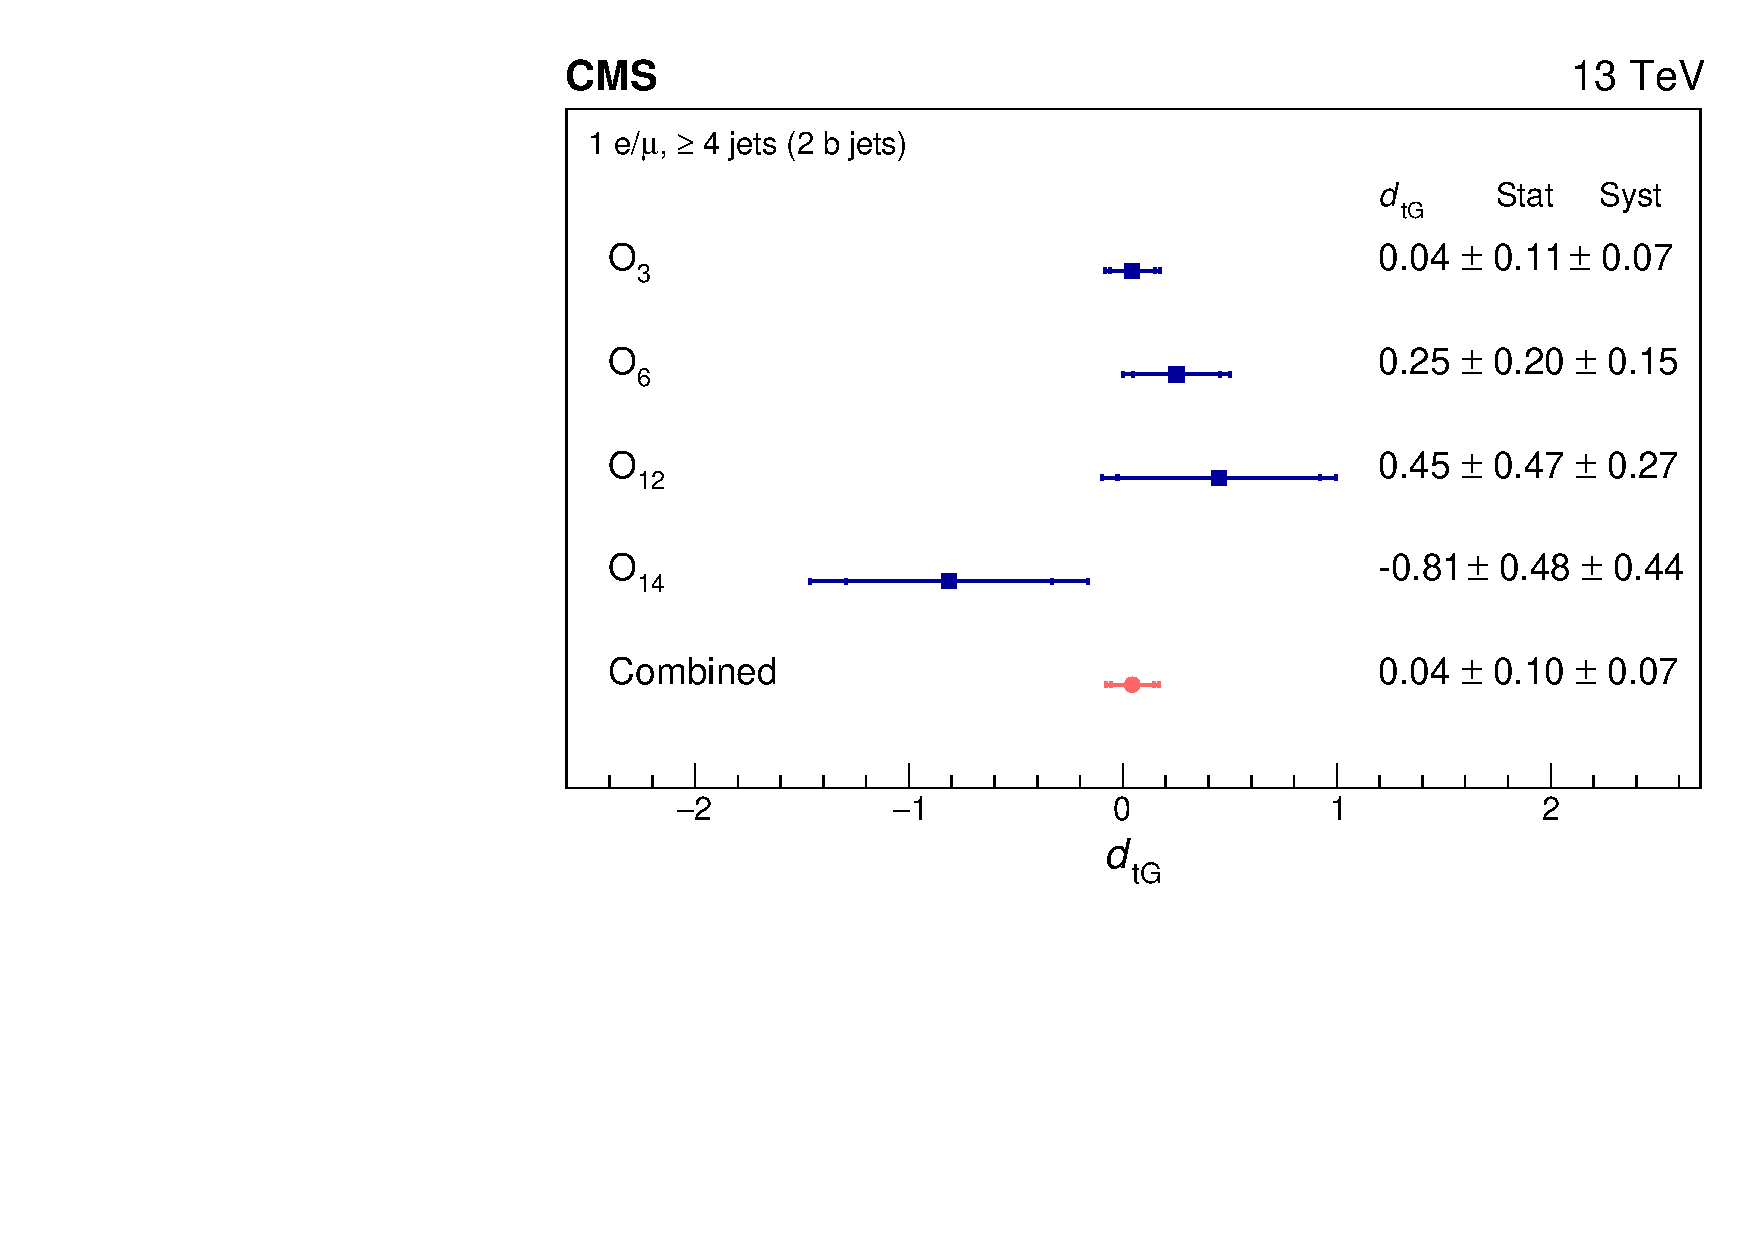
\includegraphics[width=0.8\textwidth]{figure/cedm_combined_results.pdf}
    \caption[The measured dimensionless CEDM \dtG for each CP observable.]
    {
        The measured dimensionless CEDM \dtG for each CP observable (blue squares) in the lepton+jets channel and the combined result (red point).
        The inner horizontal bars on the points represent the statistical uncertainty and the outer bar the combined statistical and systematic uncertainties added in quadrature.
    }
    \label{fig:upper_limit}
\end{figure}

Constraints on the CEDM of the top quark have also been set by CMS from measurements of the spin correlations~\cite{CPVtop:spin_correlation} in dilepton \ttbar events using \dt, which is the dimensionless parameter of CEDM in the convention of Ref.~\cite{Bernreuther:2013aga}.
The relation between \dt and \dtg can be expressed as $\dt=\Mt \dtg$~\cite{CPVtop:spin_correlation_dtg}.
From Eq.~\eqref{eq:cedm_conversion}, with the BSM scale $\Lambda$ at 1\TeV, the combined \dtG values from this analysis can be converted into a 95\% \CL limit of $\abs{\dt} < 0.015$.
This is competitive with the 95\% \CL limits obtained by the spin-correlation measurement~\cite{CPVtop:spin_correlation} of $-0.020 < \dt < 0.012$.
